\section{Diagrams}

Figure \ref{fig:cons} presents the constellation diagrams derived from the dataset utilized in our research. Each diagram includes a sample from each class along with their corresponding randomly generated noise. The diagrams depict the signal as a two-dimensional scatter plot in the complex plane at symbol sampling instants. Additionally, we provide the noiseless images to illustrate the original signal without noise. The list of classes are provided in Table \ref{tab:classes}.

\begin{table}[h]
    \centering
    \caption{List of classes in the diagram}
    \begin{tabular}{|c|c|}
        \hline
        Class Number & Class Name \\ \hline
        1 & 4ASK \\ \hline
        2 & 4PAM \\ \hline
        3 & 8ASK \\ \hline
        4 & 16PAM \\ \hline
        5 & CPFSK \\ \hline
        6 & DQPSK \\ \hline
        7 & GFSK \\ \hline
        8 & GMSK \\ \hline
        9 & OOK \\ \hline
        10 & OQPSK \\ \hline
    \end{tabular}
    \label{tab:classes}
\end{table}

Figure \ref{fig:radio} illustrates the RadioML diagram, which is used to visualize the performance of machine learning models in radio signal classification tasks. This diagram helps in understanding how well the model can distinguish between different types of radio signals.

\begin{figure*}[hbp]
    \centering
    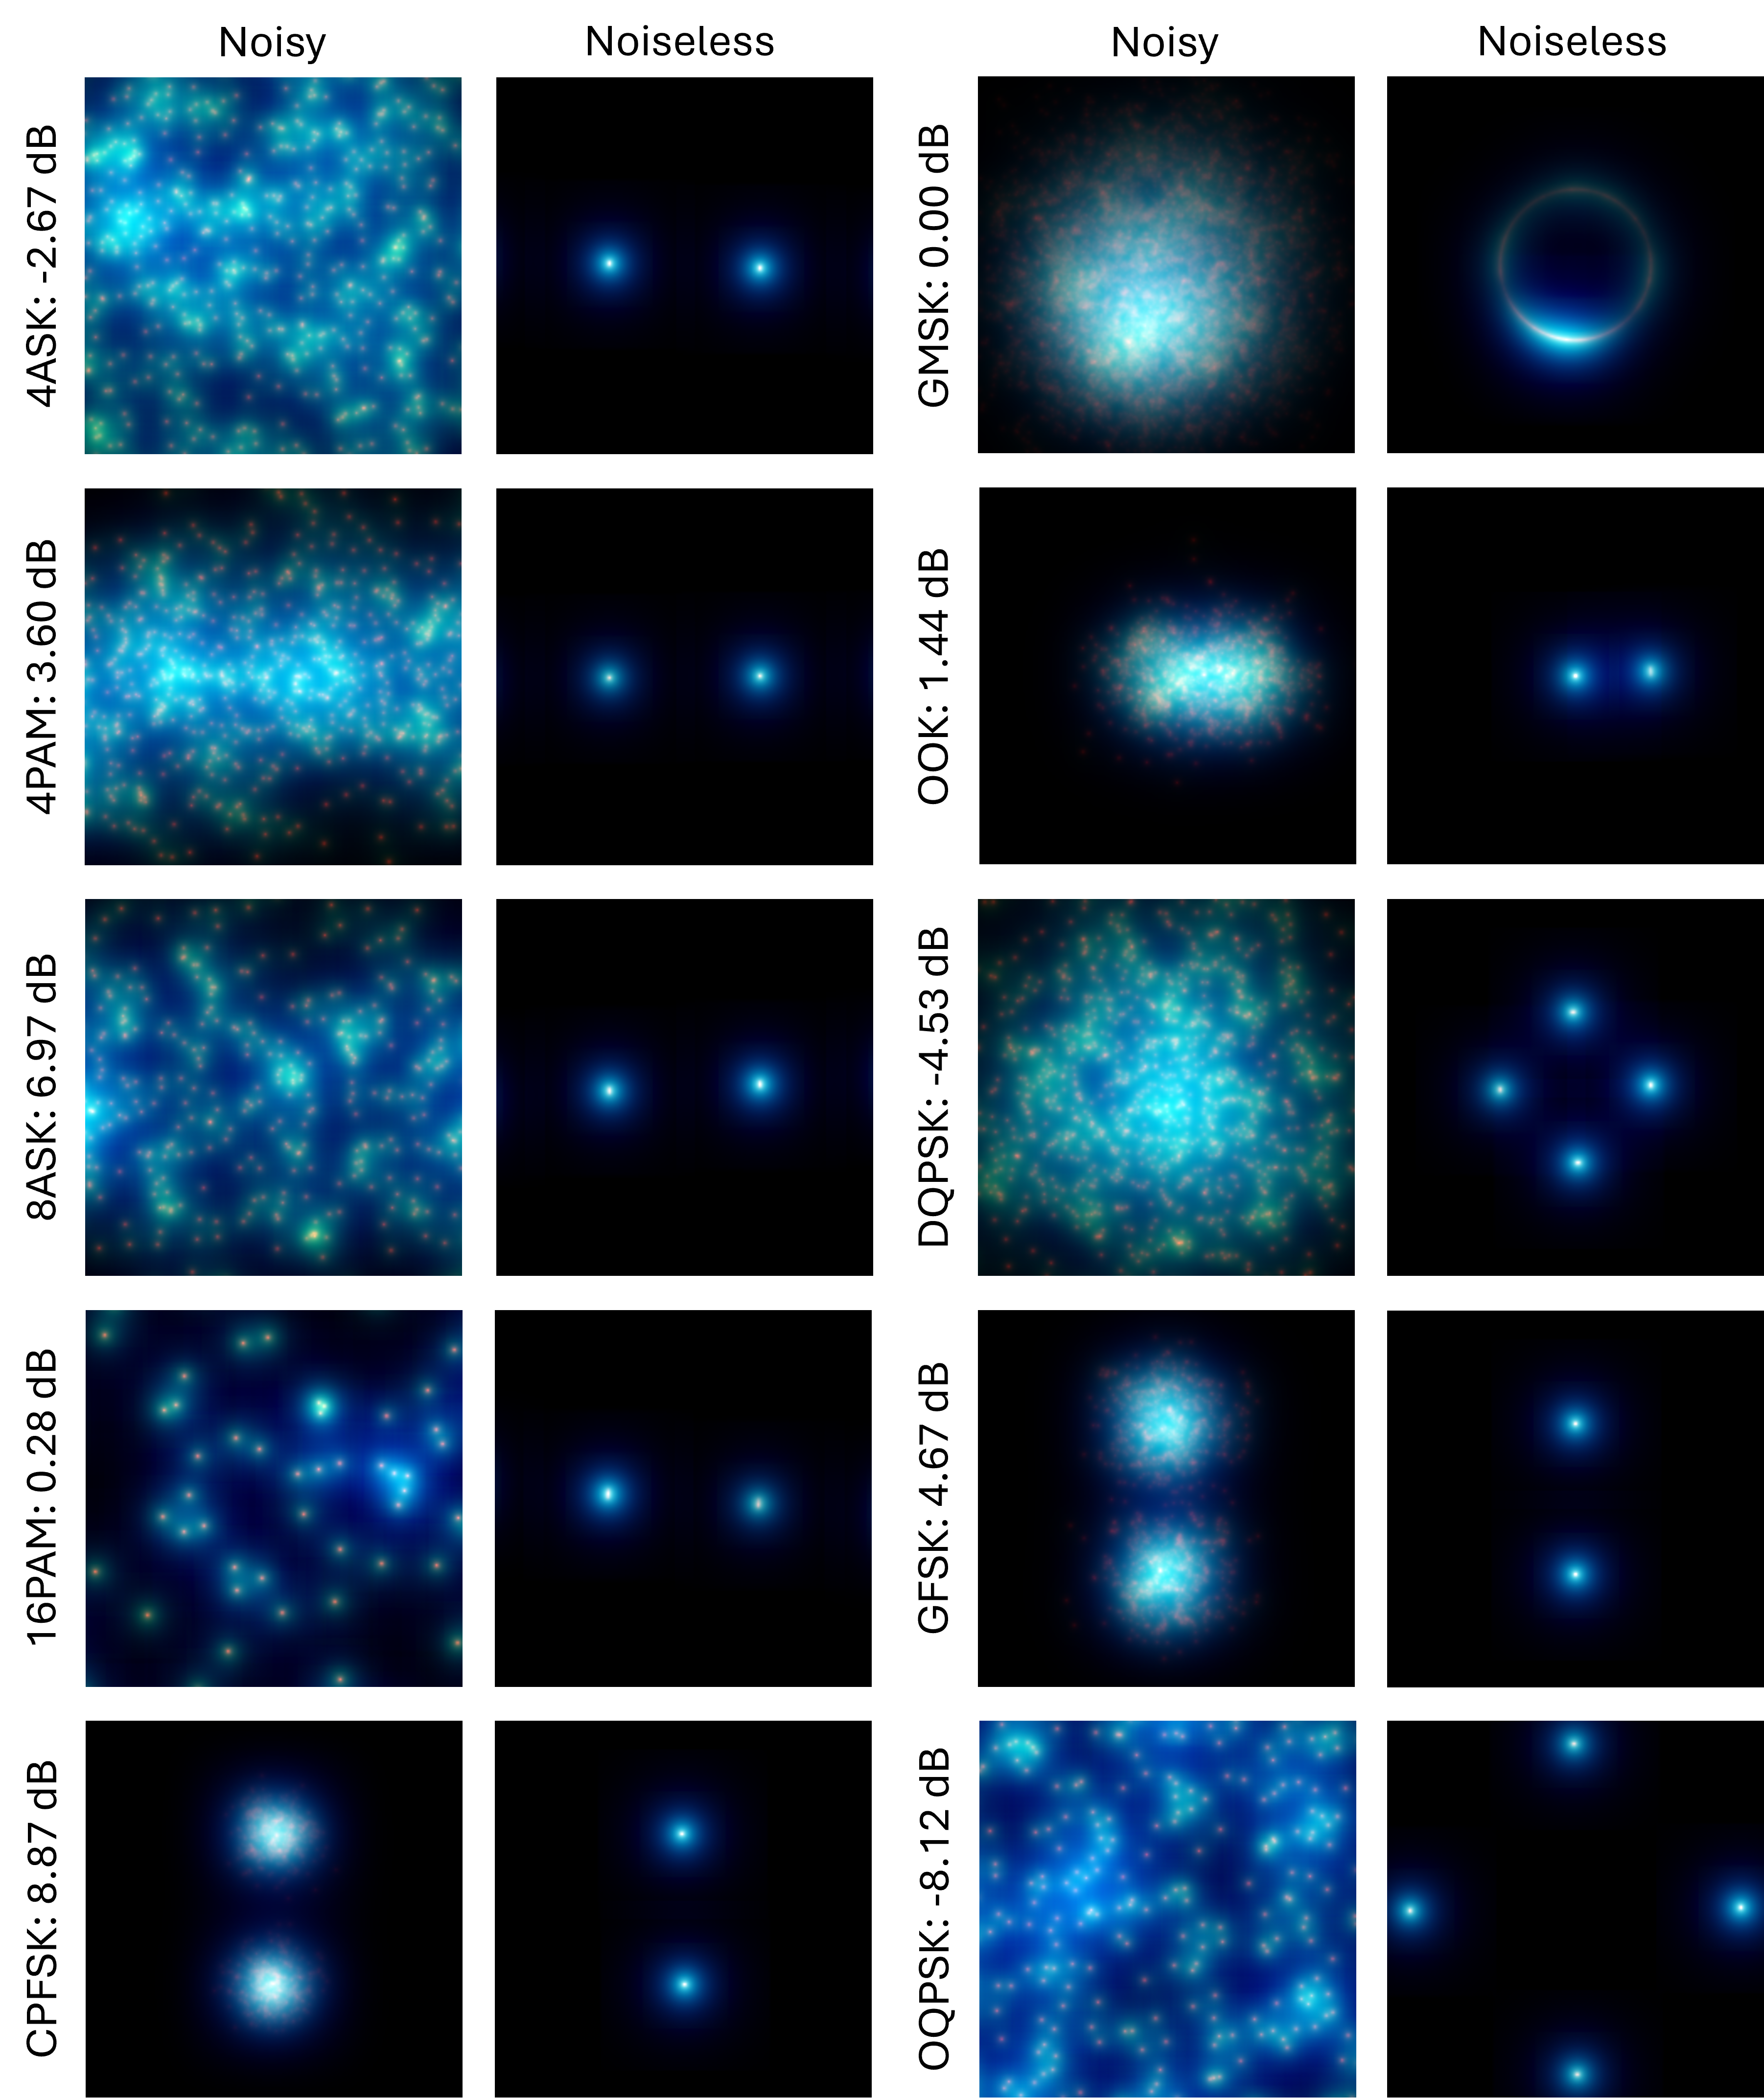
\includegraphics[width=0.8\linewidth]{images/cons.png}
    \caption{constellation diagram}
    \label{fig:cons}
\end{figure*}


\begin{table}[h]
    \centering
    \caption{List of classes in the RadioML diagram}
    \begin{tabular}{|c|c|}
        \hline
        Class Number & Class Name \\ \hline
        1 & 4ASK \\ \hline
        2 & 8ASK \\ \hline
        3 & 8PSK \\ \hline
        4 & 16APSK \\ \hline
        5 & 16PSK \\ \hline
        6 & 16QAM \\ \hline
        7 & 32APSK \\ \hline
        8 & 32QAM \\ \hline
        9 & 64APSK \\ \hline
        10 & 64QAM \\ \hline
        11 & 128APSK \\ \hline
        12 & 128QAM \\ \hline
        13 & 256QAM \\ \hline
        14 & AM-DSB-SC \\ \hline
        15 & AM-DSB-WC \\ \hline
        16 & AM-SSB-SC \\ \hline
        17 & AM-SSB-WC \\ \hline
        18 & BPSK \\ \hline
        19 & FM \\ \hline
        20 & GFSK \\ \hline
        21 & OQPSK \\ \hline
        22 & OOK \\ \hline
        23 & OQPSK \\ \hline
        24 & QPSK \\ \hline
    \end{tabular}
    \label{tab:radioml_classes}
\end{table}


\begin{figure*}[htbp]
    \centering
    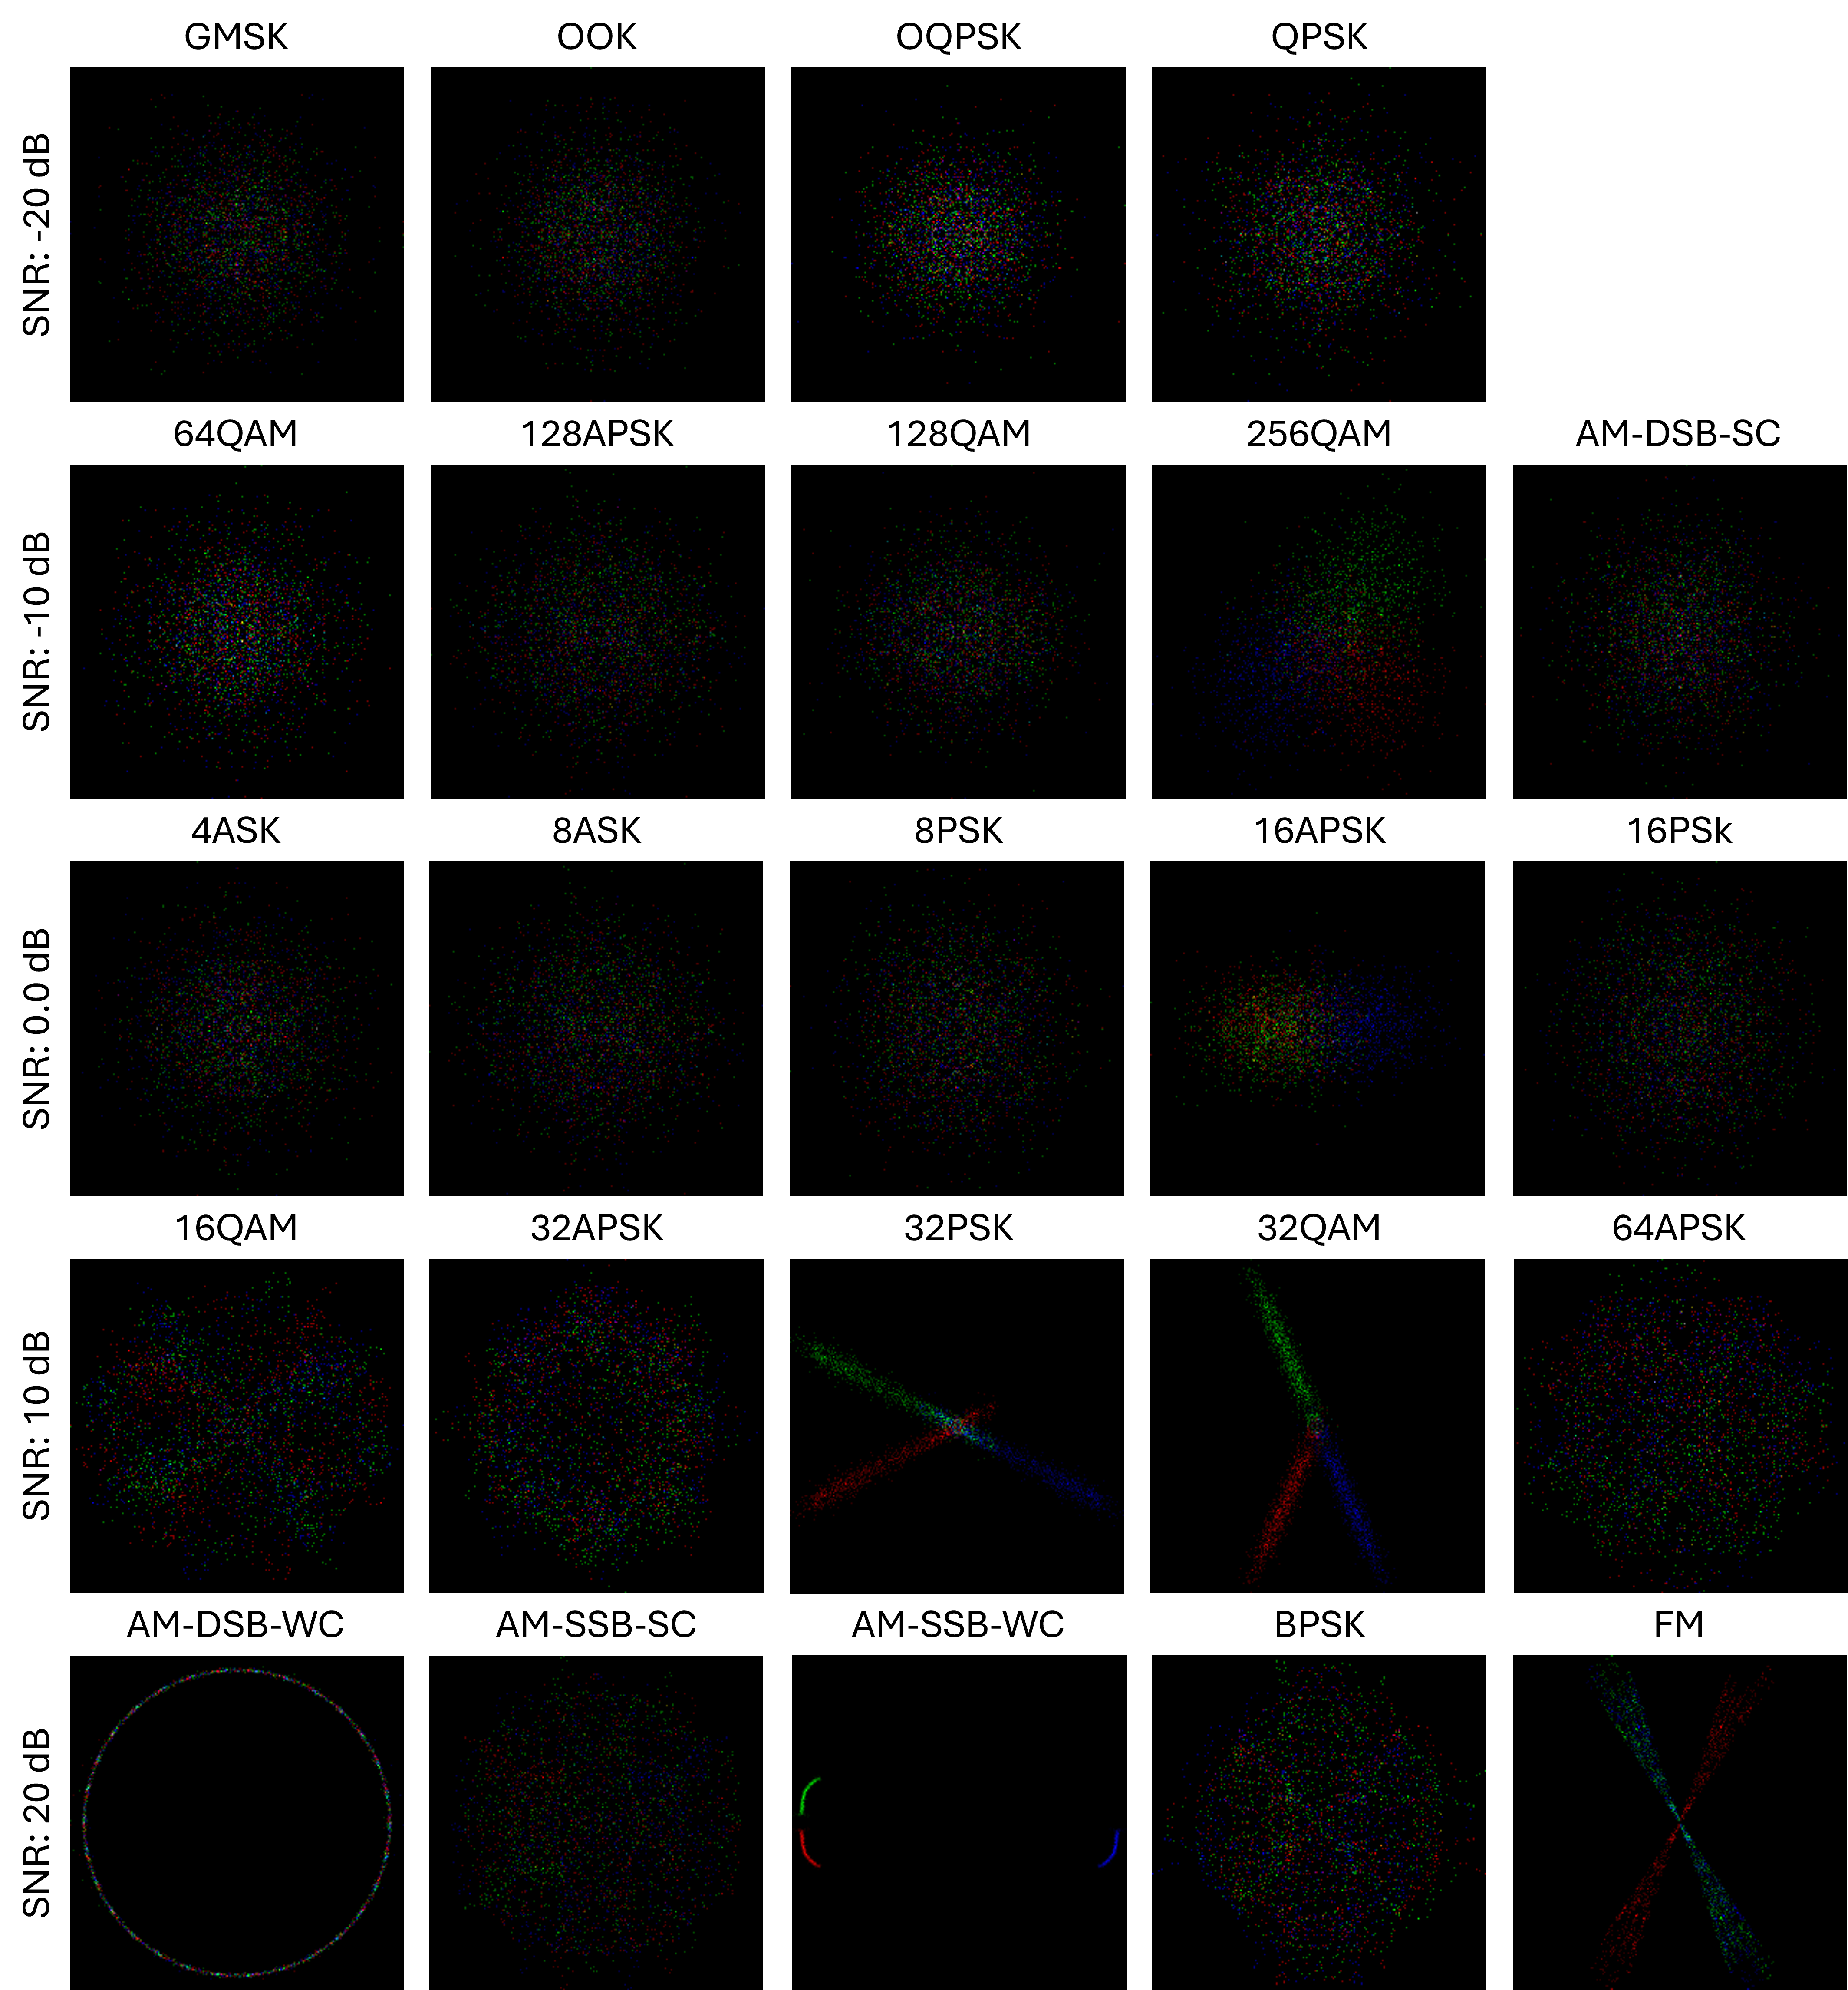
\includegraphics[width=0.8\linewidth]{images/radio.png}
    \caption{RadioML diagram}
    \label{fig:radio}
\end{figure*}

\section{List of hyperparameter During Pretraining}

\begin{table}[h]
    \centering
    \caption{List of hyperparameters during pretraining}
    \begin{tabular}{|c|c|}
        \hline
        \textbf{Parameter name} & \textbf{Value} \\ \hline
        Training batch size & 64 \\ \hline
        Testing batch size & 10 \\ \hline
        Image size & 224, 224 \\ \hline
        Patch size & 16 \\ \hline
        Mask ratio & 0.75 \\ \hline
        Encoder embedding dimension & 768 \\ \hline
        Decoder embedding dimension & 512 \\ \hline
        Encoder depth & 12 \\ \hline
        Decoder depth & 8 \\ \hline
        Encoder number of heads & 12 \\ \hline
        Decoder number of heads & 8 \\ \hline
        Number of epochs & 100 \\ \hline
        Learning rate & 0.0003 \\ \hline
        Weight decay & 0.05 \\ \hline
        Classification loss weight & 0.1 \\ \hline
        Reconstruction loss weight & 1.0 \\ \hline
    \end{tabular}
    \label{tab:pre_para}
\end{table}

\section{List of hyperparameter During Finetuning}

\begin{table}[h]
    \centering
    \caption{List of hyperparameters during pretraining}
    \begin{tabular}{|c|c|}
        \hline
        \textbf{Parameter name} & \textbf{Value} \\ \hline
        Training batch size & 32 \\ \hline
        Testing batch size & 10 \\ \hline
        Image size & 224, 224 \\ \hline
        Patch size & 16 \\ \hline
        Encoder embedding dimension & 768 \\ \hline
        Encoder depth & 12 \\ \hline
        Encoder number of heads & 12 \\ \hline
        Number of epochs & 150 \\ \hline
        Learning rate & 0.0001 \\ \hline
        Weight decay & 0.05 \\ \hline
        Number of classes & 10, 24 \\ \hline
    \end{tabular}
    \label{tab:fine_para}
\end{table}

\section{More Denoising Examples}

\begin{table*}[htbp]
    \centering
    \caption{Comparison of DenoMAE2.0 with other modulation classification methods}
    \label{compare}
    \begin{tabular}{cccccc}
    \toprule
    \multirow{2}{*}{\textbf{Methods}} & \multicolumn{2}{c}{\textbf{Number of samples}} & \multirow{2}{*}{\textbf{SNR dB}} & \multirow{2}{*}{\textbf{Number of classes}} & \multirow{2}{*}{\textbf{Test accuracy (\%)}} \\ 
    \cmidrule(lr){2-3}
     & \textbf{Pretraining} & \textbf{Fine-tuning} & & \\ \midrule
    
    AlexNet \cite{peng2018modulation}  & 800,000 (train) & 8,000 (test)  & 2 & 8 & 82.8  \\
    NMformer \cite{faysal2024nmformer} & 106,800 & 3,000 & 0.5 - 4.5 & 10 & 71.6 \\
    CNN-AMC \cite{meng2018automatic} & 79,200 & 228,060 & -6 & 4 & 50.40 \\
    DL-GRF \cite{sun2022automatic} &  2,000 (train) & 200 (test) & 0 & 4 & 59 \\
    DenoMAE \cite{faysal2025denomae} & 10,000 & 1,000 & 0 - 10 & 10 & 81.3 \\
    DenoMAE2.0 (\textbf{Ours}) & 10,000 & 1,000 & 0 - 10 & 10 & 82.4 \\
    
    \bottomrule
    \end{tabular}
\end{table*}

\section{Comparison with Other Methods}